\documentclass{article}
\usepackage{blindtext}
\usepackage[a4paper, total={6in, 8in}]{geometry}
\usepackage{graphicx} % Required for inserting images
\usepackage{amsmath}
\usepackage{doi}

\newcommand{\dd}[1]{\mathrm{d}#1}

\title{Two-State Model of Backtracking Rescue by GreB}
\author{Xiang Gao}
\date{September 2024}

\begin{document}
\maketitle

In the presence of GreB, GreB may rescue a backtracked RNA polymerase (RNAP) and bring it into active elongation. Thus the stalling process consists of transitions from two states: backtracking and active elongation. The stochastic transitions between the two states may be described as reversible first-order reactions with reaction rates $k_-$ and $k_+$, corresponding to the transition rate from elongation state to backtracking state and the transition rate from backtracking state to elongation state, respectively. \\
\begin{center}
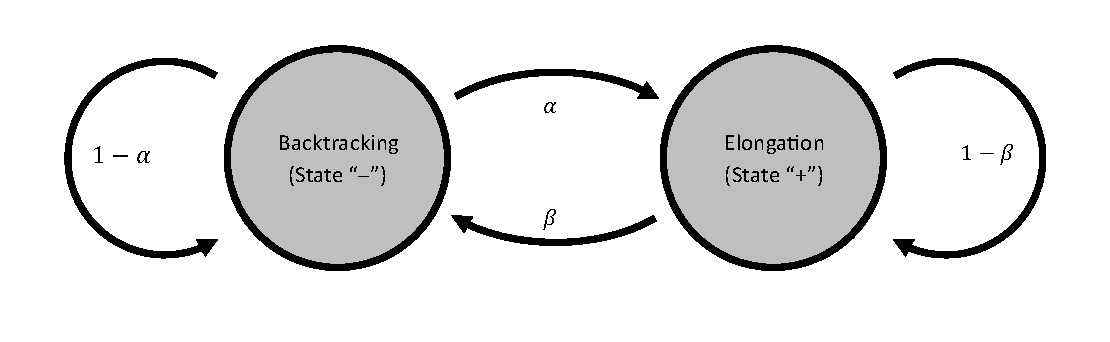
\includegraphics[scale=0.5]{si_figure_plain} \\
\end{center} 
During backtracking, RNAP moves at a velocity $v_-$, during active elongation, it moves at a velocity $v_+$. We sought to determine $k_-$ and $k_+$ in terms of measured RNAP positions and measured velocities $v_-$ and $v_+$. \\

\section{Markov model}
We first considered these two-state transitions during an infinitely small time interval ${\Delta}t$ (figure). During this time, the probabilities of transitioning from ‘-’ to a ‘+’ state and from ‘$+$’ to ‘$-$’ state are ${\alpha}=k_+{\cdot}{\Delta}t$ and ${\beta}=k_-{\cdot}{\Delta}t$ respectively. \\
These transitions follow the Markov process and the probabilities being in the ‘+’ and ‘-’ states evolve as \\

\begin{equation}
    \begin{pmatrix} P_-^{(i+1)} \\ P_+^{(i+1)} \end{pmatrix} 
    = 
    \begin{pmatrix} 1 - \alpha & \beta \\ \alpha & 1 - \beta \end{pmatrix} 
    \begin{pmatrix} P_-^{(i)} \\ P_+^{(i)} \end{pmatrix}
\end{equation}  \\

with the transition matrix: \\

\begin{equation}
    T=\begin{pmatrix}  
    {1-\alpha} & \beta \\  \alpha & {1-\beta}
    \end{pmatrix}
\end{equation} \\

\section{The eigenvalues and eigenvectors of transition matrix}
The eigenvalues and eigenvectors of the transition matrix can be calculated as follows

\begin{equation}
    0=T-{\lambda}I=\begin{pmatrix} 1 - \alpha - \lambda & \beta \\ \alpha & 1 - \beta - \lambda \end{pmatrix}
\end{equation} \\

The two eigenvalues are ${\lambda}_1=1$ and ${\lambda}_2=1-\alpha-\beta$. It is worth noting that 
$1-\alpha-\beta \subset(-1,1)$. \\

The eigenvectors satisfy: \\

\begin{equation}
    T\boldsymbol{V_k}={\lambda}_k\boldsymbol{V_k}
\end{equation}

where $V_k$ is the $k$-th eigenvector ($k$ = 1,2) that corresponds to ${\lambda}_k$ . We find the eigenvectors by
solving Eq. 4: \\

\begin{equation}
    \boldsymbol{V_1}=\begin{pmatrix}
        \beta \\ \alpha
    \end{pmatrix},
    \boldsymbol{V_2}=\begin{pmatrix}
        1 \\ -1
    \end{pmatrix}
\end{equation}

We define: \\

\begin{equation}
    \Lambda=\begin{pmatrix}
        {\lambda}_1 & 0 \\ 0 & {\lambda}_2
    \end{pmatrix},
    V=\begin{pmatrix}
        \boldsymbol{V_1} & \boldsymbol{V_2}
    \end{pmatrix}
\end{equation}

\begin{equation}
    TV=T\begin{pmatrix}
        \boldsymbol{V_1} & \boldsymbol{V_2}
    \end{pmatrix}=
    \begin{pmatrix}
        {\lambda}_1\boldsymbol{V_1} & {\lambda}_2\boldsymbol{V_2}
    \end{pmatrix}=
    \begin{pmatrix}
        \boldsymbol{V_1} & \boldsymbol{V_2}
    \end{pmatrix}\Lambda=
    V\Lambda
\end{equation} \\

Therefore \\

\begin{equation}
T=V\Lambda V^{-1}
\end{equation}

and \\

\begin{equation}
T^N=V{\Lambda}^N V^{-1}
\end{equation}

At the time $t$, $N=t/{\Delta t}$ number of $\Delta t$ steps will have been taken. The $N$-step transition matrix can be written as: \\

\begin{equation}
    \begin{aligned}
    T^N &=V\Lambda^N V^{-1} \\
        &=\frac{1}{\alpha + \beta} \begin{pmatrix} \beta & 1 \\ \alpha & -1 \end{pmatrix} 
            \begin{pmatrix} 1 & 0 \\ 0 & (1 - \alpha - \beta)^N \end{pmatrix} 
            \begin{pmatrix} 1 & 1 \\ \alpha & -\beta \end{pmatrix} \\
        &=\frac{1}{\alpha + \beta}
            \begin{pmatrix} 
                \beta + s \alpha & \beta - s \beta \\
                \alpha - s \alpha & \alpha + s \beta 
            \end{pmatrix}\
    \end{aligned}
\end{equation} \\

where $s=(\alpha+\beta-1)^N$. When $N\rightarrow\infty$ and $s\rightarrow 0$ \\

\begin{equation}
    T^{\infty}=\dfrac{1}{\alpha+\beta} \begin{pmatrix}
        \beta & \beta \\ \alpha & \alpha
    \end{pmatrix}
\end{equation}

which gives the probabilities when the two states are under equilibrium and is independent of
the initial states. \\

\section{Velocity correlation}
Although we ultimately wished to find the solution of position correlation, it was mathematically more conducive to start by finding the velocity correlation. We assumed that at the starting point of measurement, the system is in equilibrium. The velocity correlation between the initial state and the $N$th-step can be written as $\langle v_0 v_N \rangle$, which equals to the average of all possible combinations of correlation of stochastic velocity variables, e.g., \\


\begin{equation}
    \begin{aligned}
        \langle v_0 v_N \rangle 
        &=
            v_- P_-^{\infty} 
                \begin{pmatrix}
                    v_- & v_+
                \end{pmatrix}
                \begin{pmatrix}
                    P_{(-|-)}^N \\ P_{(+|-)}^N
                \end{pmatrix} 
            +
            v_+ P_+^{\infty}
                \begin{pmatrix}
                    v_- & v_+
                \end{pmatrix}
                \begin{pmatrix}
                    P_{(-|+)}^N \\ P_{(+|+)}^N
                \end{pmatrix} \\
        &=
            \begin{pmatrix}
                v_- & v_+
            \end{pmatrix} T^N 
        \begin{pmatrix} v_- P_-^{\infty} \\ v_+ P_+^{\infty} \end{pmatrix}
    \end{aligned}
\end{equation}  \\

where $P_-^{\infty}$ and $P_+^{\infty}$ are the probabilities of state '-' and '+' at 0-th step respectively. $P_{(i|j)}^N$ is the conditional probability that the state is $j$ at 0-th step and the state becomes $i$ after N steps. \\
Plugging $T^N$ $P_-^{\infty}$, and $P_+^{\infty}$ into Eq. 12, we have

\begin{equation}
    \langle v_0 v_N \rangle=
    \frac{1}{\alpha + \beta}
    \begin{pmatrix} v_- & v_+\end{pmatrix}
    \begin{pmatrix} 
        \beta + s \alpha & \beta - s \beta \\ \alpha - s \alpha & \alpha + s \beta 
    \end{pmatrix}
    \begin{pmatrix} 
        v_- \beta / (\alpha + \beta) \\
        v_+ \alpha / (\alpha + \beta)
    \end{pmatrix}
\end{equation}

To convert this expression to a continuous form, we take the limit that the time step interval $\Delta t \rightarrow 0$. We have thus obtained the velocity correlation as a function of time

\begin{equation}
    \langle v_0 v_N \rangle=A+Be^{-kt}
\end{equation}

where $A=(\frac{k_- v_- + k_+ v_+}{k_- + k_+})^2$, $B=k_- k_+ (\frac{v_- - v_+}{k_- + k_+})^2$, and $k=k_- + k_+$.

\section{Position correlation}

We assume that all position trajectories, $x(t)$, are the samples from the same ensemble, therefore:

\begin{equation}
    \begin{aligned}
    \langle (x(t) - x(0))^2 \rangle 
    &= \langle ( \int_0^t v(t_1) dt_1 )^2 \rangle  
    = \int_0^t \int_0^t \left\langle v(t_1) v(t_2) \right\rangle dt_1 dt_2 \\
    &= \int_0^t \int_0^t \left\langle v(0) v(|t_2 - t_1|) \right\rangle dt_1 dt_2 \\
    &= \int_0^t \int_0^t \left[ A + B e^{-k|t_2 - t_1|} \right] dt_1 dt_2 \\
    &= 2 \int_0^t dt_2 \int_0^{t_2} \left[ A + B e^{-k(t_2 - t_1)} \right] dt_1 \\
    &= At^2 + \frac{2B}{k} t - \frac{2B}{k^2} \left[ 1 - e^{-kt} \right] 
    \end{aligned}
\end{equation}

It is worth noting that line 2 of Eq. 15 assumes that the system has already reached
equilibrium at the time $t=0$, so $\langle v(t_1)v(t_2)\rangle = \langle v(0) v(\left| t_2 - t_1 \right|\rangle$. This is true in practice since at $t=0$, we only know the probabilities that RNAP is in either an elongation state or backtracking state. \\
In Eq. 15, the first term is a linear drift of the mean position:

\begin{equation}
    \bar{x}(t)=\frac{k_- v_- + k_+ v_+}{k_- + k_+}
\end{equation} 

Therefore, variance of the position is

\begin{equation}
    \sigma_x^2(t)=\langle ( x(t) - x(0))^2 \rangle - \langle x(t) \rangle ^2 
    = \frac{2B}{k}t - \frac{2B}{k^2}[1-e^{-kt}]
\end{equation}

When $kt\gg1$, the variance evolves with time as follows

\begin{equation}
    \sigma_x^2(t)=\frac{2B}{k}t
    = \frac{2k_- k_+}{{k_- + k_+}^3}(v_- - v_+)^2ts
\end{equation}

\section*{Reference}
Ma J, Tan C, \textbf{Gao X}, Fulbright RM, Roberts JW, Wang MD. Transcription factor regulation of RNA polymerase’s torque generation capacity. \emph{Proceedings of the National Academy of Sciences of the United States of America}. 2019 Feb 12;116(7):2583-8. \doi{10.1073/pnas.1807031116}

\end{document}
